\documentclass[11pt]{article}
\usepackage[
style=authoryear,
]{biblatex}
\addbibresource{biblio.bib} 
%prepared in AMSLaTeX, under LaTeX2e
\addtolength{\oddsidemargin}{-.75in} 
\addtolength{\evensidemargin}{-.75in}
\addtolength{\topmargin}{-.6in}
\addtolength{\textwidth}{1.4in}
\addtolength{\textheight}{1.3in}
\renewcommand{\baselinestretch}{1.06}

\usepackage{wrapfig,fancyvrb,xspace}
\usepackage{palatino,amsmath,amssymb,amsthm,bm}
\usepackage[final]{graphicx}
\usepackage[pdftex, colorlinks=true, plainpages=false, linkcolor=blue, citecolor=red, urlcolor=blue]{hyperref}

% macros
\newcommand{\bn}{\mathbf{n}}
\newcommand{\bq}{\mathbf{q}}
\newcommand{\bu}{\mathbf{u}}
\newcommand{\bw}{\mathbf{w}}
\newcommand{\bx}{\mathbf{x}}

\newcommand{\bX}{\mathbf{X}}

\newcommand{\cH}{\mathcal{H}}
\newcommand{\cK}{\mathcal{K}}
\newcommand{\cV}{\mathcal{V}}

\newcommand{\RR}{\mathbb{R}}

\newcommand{\Div}{\nabla\cdot}
\newcommand{\eps}{\epsilon}
\newcommand{\grad}{\nabla}
\newcommand{\lam}{\lambda}

\newcommand{\ds}{\displaystyle}


\title{A porous media test case in Firedrake}
\author{Ed Bueler}
\date{\today}

\begin{document}
\maketitle
%\begin{abstract}
%FIXME
%\end{abstract}

\thispagestyle{empty}

\section{A (draft) porous medium model for Darcy-type gas flow}

Suppose $\Omega$ is a 2-dimensional domain such as a square.  We will use $x$ for the horizontal and $z$ for the vertical coordinate.  We assume $z$ is measured positive upward.  Within $\Omega$ we assume there is a matrix of porous material with variable properties of porosity $\phi(x,z)$ and permeability $k(x,z)$; these are assumed independent of time.

A gas flows through that medium.  We will take various properties of the gas to be positive constants: $\mu$ is the dynamic viscosity, $R$ is the gas constant, $T$ is the absolute temperature, and $M$ is the molar mass.  The following system of equations, a mathematical model, applies to determing the evolution of the density $\rho(t,x,z)$, pressure $P(t,x,z)$, and vector volumetric flux $\bq(t,x,z)$:\footnote{TS: Please check that this is the model you want?}
\begin{subequations}
\label{eq:pmtime:early}
\begin{align}
\frac{\partial}{\partial t} \left(\rho \phi\right) + \Div \left(\rho\, \bq\right) &= 0 \label{eq:masscont} \\
\bq &= - \frac{k}{\mu} \grad\left(P + \rho g z\right) \label{eq:darcy} \\
\rho &= \frac{M}{RT} P \label{eq:idealgas}
\end{align}
\end{subequations}

Regarding the above system we can make comments.  To be physical the density must be non-negative: $\rho\ge 0$.  We are assuming no mass sources or sinks in \eqref{eq:masscont}, otherwise there could be a function on the right.  From the static pressure $P_0=-\rho g z$ note that $P+\rho g z = P-P_0$, we see that the flow in \eqref{eq:darcy} is driven by deviations from static pressure.  The volumetric flux $\bq$ is related to the vector velocity $\bu$ by $\bq = \phi \bu$.  (Velocity may be helpful in diagnosing the solution but it is not needed to state the above.)

It is straightforward to eliminate $\bq$ and $P$, using also the time-independence of $\phi$.  We also simplify the name of the nontrivial ideal gas law constant:
\begin{equation}
c = \frac{RT}{M}.  \label{eq:crename}
\end{equation}
Thus:
\begin{equation}
\phi \frac{\partial \rho}{\partial t} - \frac{1}{\mu} \Div \left(k \rho \grad\left(c \rho + \rho g z\right)\right) = 0.  \qquad \text{\emph{(porous medium equation)}} \label{eq:pmtime}
\end{equation}
This form is comparable to the better-known heat equation
\begin{equation}
\frac{\partial u}{\partial t} - \Div(\grad u) = 0. \qquad \text{\emph{(heat equation)}}\label{eq:heattime}
\end{equation}

An important property of heat equation \eqref{eq:heattime} is that at each time the operator $\Div \grad = \grad^2$ acts as a kind of invertible matrix, which assists in finding the solution $u$.  Since $\rho$ appears as a flux coefficient in the porous medium equation, i.e.~the copy of $\rho$ just inside the divergence in \eqref{eq:pmtime}, this invertibility will be lost if $\rho\to 0$ somewhere.  This is called ``degeneration'' of the diffusivity.  It is a well-known property of the porous medium equation which must be taken seriously when solving numerically.


\section{Steady state test cases}

The porous medium equation \eqref{eq:pmtime} is time dependent.  It has an obvious steady-state form found by setting $\partial \rho/\partial t = 0$:
\begin{equation}
- \Div \left(k \rho \grad\left(c \rho + \rho g z\right)\right) = 0 \label{eq:pm:strong}
\end{equation}
In equation \eqref{eq:pm:strong}, the strong form, the scalar function $\rho(x,z)$ is unknown.  Note that $\phi,\mu$ are not parameters in this time-independent and source-free situation.  

To derive the weak form we first multiply by a test function $w(x,z)$ and integrate over $\Omega$:
    $$\int_\Omega- \Div \left(k \rho \grad\left(c \rho + \rho g z\right)\right) w = 0.$$
Integration by parts, i.e.~the product rule plus the divergence theorem, gives:
\begin{equation}
- \int_{\partial\Omega} k \rho w \grad\left(c \rho + \rho g z\right) \cdot \bn + \int_\Omega k \rho \grad\left(c \rho + \rho g z\right) \cdot \grad w = 0.\label{eq:pm:preliminaryweak}
\end{equation}
Equation \eqref{eq:pm:preliminaryweak} is a preliminary weak form, into which we must put some boundary conditions.\footnote{TS: I have no idea what boundary conditions you want, actually.}

For now here are two proposed, concrete test cases.  Here $\Omega$ is the unit square $0<x<1,0<z<1$.  Matching the Firedrake convention from \texttt{UnitSquareMesh()}, the sides are indexed (1,2,3,4) for (left,right,bottom,top) respectively.

\begin{enumerate}
\item On the top side of the square $\Omega$, suppose the density has a known value of one.  On the sides and the base let us assume there is no flux.  Thus
\begin{subequations}
\begin{align}
\rho &= 1 & &(4=\text{top}) \label{eq:onebc:dirichlet} \\
\bq \cdot \bn = - \frac{k}{\mu} \grad(c\rho + \rho g z) \cdot \bn &= 0 & &(1,2,3=\text{left},\text{right},\text{bottom}) \label{eq:onebc:noflux}
\end{align}
\end{subequations}
By \eqref{eq:onebc:noflux} the 1,2,3 parts of the boundary integral in \eqref{eq:pm:preliminaryweak} are zero, thus
	$$- \int_{\partial_4\Omega} k \rho w \grad\left(c \rho + \rho g z\right) \cdot \bn + \int_\Omega k \rho \grad\left(c \rho + \rho g z\right) \cdot \grad w = 0.$$

To enforce the condition on the top boundary $\partial_4\Omega$ we must assume that the test functions $w$ satisfy zero along there.  Denote $H_D^1(\Omega)$ for this space of test functions which are zero along the Dirichlet boundary.  The entire boundary integral is now zero, and the weak form is just
\begin{equation}
\int_\Omega k\rho \grad\left(c\rho + \rho g z\right) \cdot \grad w = 0 \qquad \text{ for all } w \in H_D^1(\Omega).\label{eq:pm:weakone}
\end{equation}
This weak form corresponds to the Firedrake/UFL code
\begin{Verbatim}[fontsize=\small]
    F = ( k * rho * dot(grad(c * rho + rho * g * z), grad(w)) ) * dx
\end{Verbatim}

\item This is a small modification of case 1.  We keep the top, bottom, and right sides the same, but suppose that there is nonzero flux into the left side:
\begin{subequations}
\begin{align}
\rho &= 1 & &(4=\text{top}) \label{eq:twobc:dirichlet} \\
\bq \cdot \bn = - \frac{k}{\mu} \grad(c\rho + \rho g z) \cdot \bn &= 0 & &(2,3=\text{right},\text{bottom}) \label{eq:twobc:noflux} \\
\bq \cdot \bn = - \frac{k}{\mu} \grad(c\rho + \rho g z) \cdot \bn &= q_1(z) & &(1=\text{left}) \label{eq:twobc:givenflux}
\end{align}
\end{subequations}
Now deriving the weak form from \eqref{eq:pm:preliminaryweak} we pick up a boundary integral:
\begin{equation}
\int_\Omega k \rho \grad\left(c\rho + \rho g z\right) \cdot \grad w + \int_{\partial_1\Omega} \mu \rho q_1 w = 0 \qquad \text{ for all } w \in H_D^1(\Omega).\label{eq:pm:weaktwo}
\end{equation}
Note that $q_1(z) = \bq \cdot \bn < 0$ corresponds to injecting gas into the left side, because $\bn = -\bx$ along that side.

For mildly interesting appearance we might set
	$$q_1(z) = \begin{cases} -c_1, & 0.2 < z < 0.4 \\ 0, & \text{otherwise} \end{cases}$$
for some value $c_1>0$.
\end{enumerate}

In the above cases the various constants are set to one, in the absence of preferred values: $k=1$, $c=1$, $\mu=1$, $g=1$.



\section{Numerical solution of the finite element equations}

Basically it is Newton's method, which is managed by the SNES component of PETSc.  Some useful options are to use the default ``line search'' Newton solver \texttt{newtonls}, and to ask for some feedback on the success/failure of the Newton steps, but to continue to solve the linear Newton step equations by LU decomposition:
\begin{Verbatim}[fontsize=\small]
    solve(F == 0, rho, bcs=[BCs],
          solver_parameters = {'snes_type': 'newtonls',
                               'snes_monitor': None,
                               'snes_converged_reason': None,
                               'ksp_type': 'preonly',
                               'pc_type': 'lu'})
\end{Verbatim}
Much more could be said.



\section{An application for the 2D Darcy-type gas flow through a porous lava dome}

In \cite{Graham2023}, we measure permeability of samples from various textural units of the Obsidian dome and South Deadman dome using field and lab permeameters. These two domes are silicic lava flows in the Inyo Craters portion of the Mono-Inyo Craters in eastern California, a chain of silicic lava flows, domes, and explosion craters that stretches 12 km (7.5 miles) to the north-northeast of Long Valley Caldera. The Inyo craters erupted as recently as ~675 years (~1350 A.D.) before present. Prior studies subdivided the majority of the lava erupted at the Inyo Craters according to the observed vesicle textures found in different parts of each flow, subdivided into finely vesicular pumice (FV), coarsely vesicular pumice (CV), and dense obsidian (OB). Shallow scientific bore hole drilling in the 1970's confirmed the presence of an underground magmatic intrusion, which was the source of the domes. This drilling also provided some general constraints on the depth of each distinct textural unit within the dome (Table \ref{tab:UnitPermPoro}).

In this study, we wish to put constraints on the surface gas flux for each textural unit at Obsidian Dome. The unit mapping of the dome is shown in Fig. \ref{fig:unitMapping}, and an example cross-section is shown in Fig. \ref{fig:crossSection}. Using constraints on dome height, the depth and permeability of each unit, and assuming a significant portion of gas is sourced from degassing of the underlying feeder dike, we can use Darcy's law to calculate the surface gas flux through each unit. This was done in \cite{Graham2023} using a 1D model of Darcy's law, as implemented in \cite{Edmonds2003}, and we wish to extend this model into 2-dimensions, to account for the unit layering, which may affect the path of gas flow towards the surface.

COMSOL model results for gas density and surface gas flux are shown in Fig. \ref{fig:COMSOLresults}, with annotations stating relevant boundary conditions. Here we assume atmospheric pressure at the surface ($P_{atm} = 1.01325$ bar) and a pressure at the base of the dome ($L=22$ m) of $P_{z=L} = 11$ bar. There is a gas inlet at the base of the CV unit, through which steam at a temperature of 920$^{\circ}$C can enter the dome porous matrix. For simplicity, a no flow condition is imposed at the unit sides, and we choose to solve for the steady-state isothermal, compressible gas flow using Darcy's Law to relate volumetric gas flux and pressure. The porosity and permeability for each unit, as well as their height and percent of total dome surface area, are shown in Table \ref{tab:UnitPermPoro}.



\begin{figure}
   \centering
\includegraphics[scale=0.3]{unitMapping.png}
\caption{Textural lithologic distribution maps of lavas for (A) Obsidian dome and (B) South Deadman dome.}
\label{fig:unitMapping}
\end{figure}

\begin{figure}
   \centering
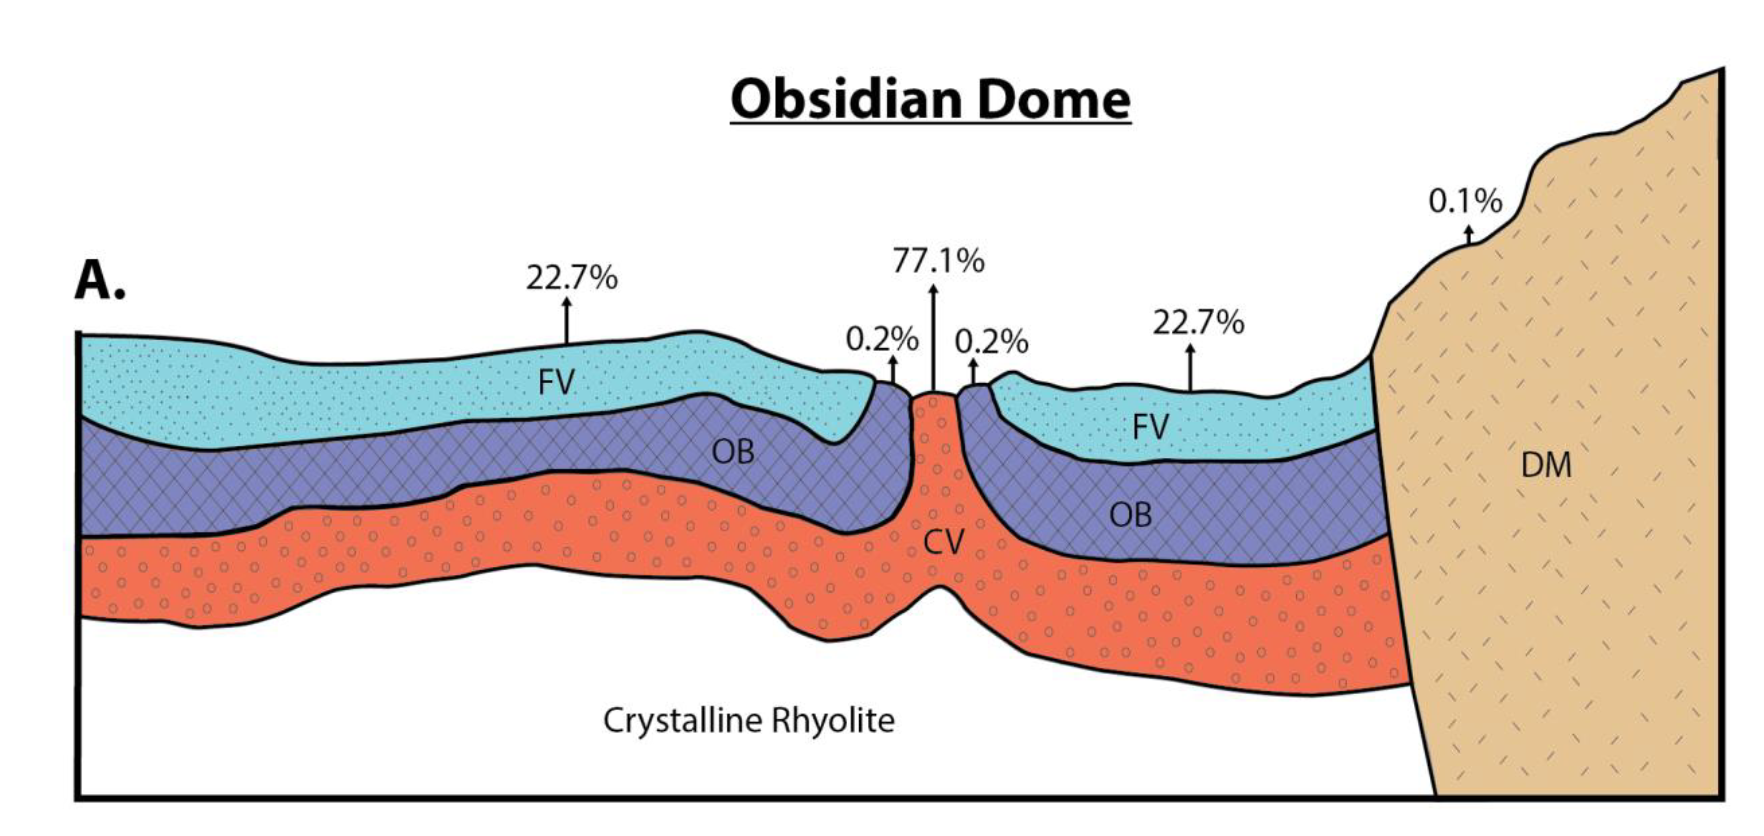
\includegraphics[scale=0.5]{crossSection.png}
\caption{Schematic diagrams depicting total calculated gas flux percentages during the final stages of lava emplacement at Obsidian dome. Total gas flux for each lithologic unit was calculated using the gas flux model of Edmonds et al. (2003), and the gas flux percentages represent the percent gas flux for each lithologic unit relative to the total gas flux calculated for all units, and does not consider additional degassing that occurs through conduit processes, fractures, tuffisite veins, or porous pathways that are too large to measure.}
\label{fig:crossSection}
\end{figure}

\begin{figure}
   \centering
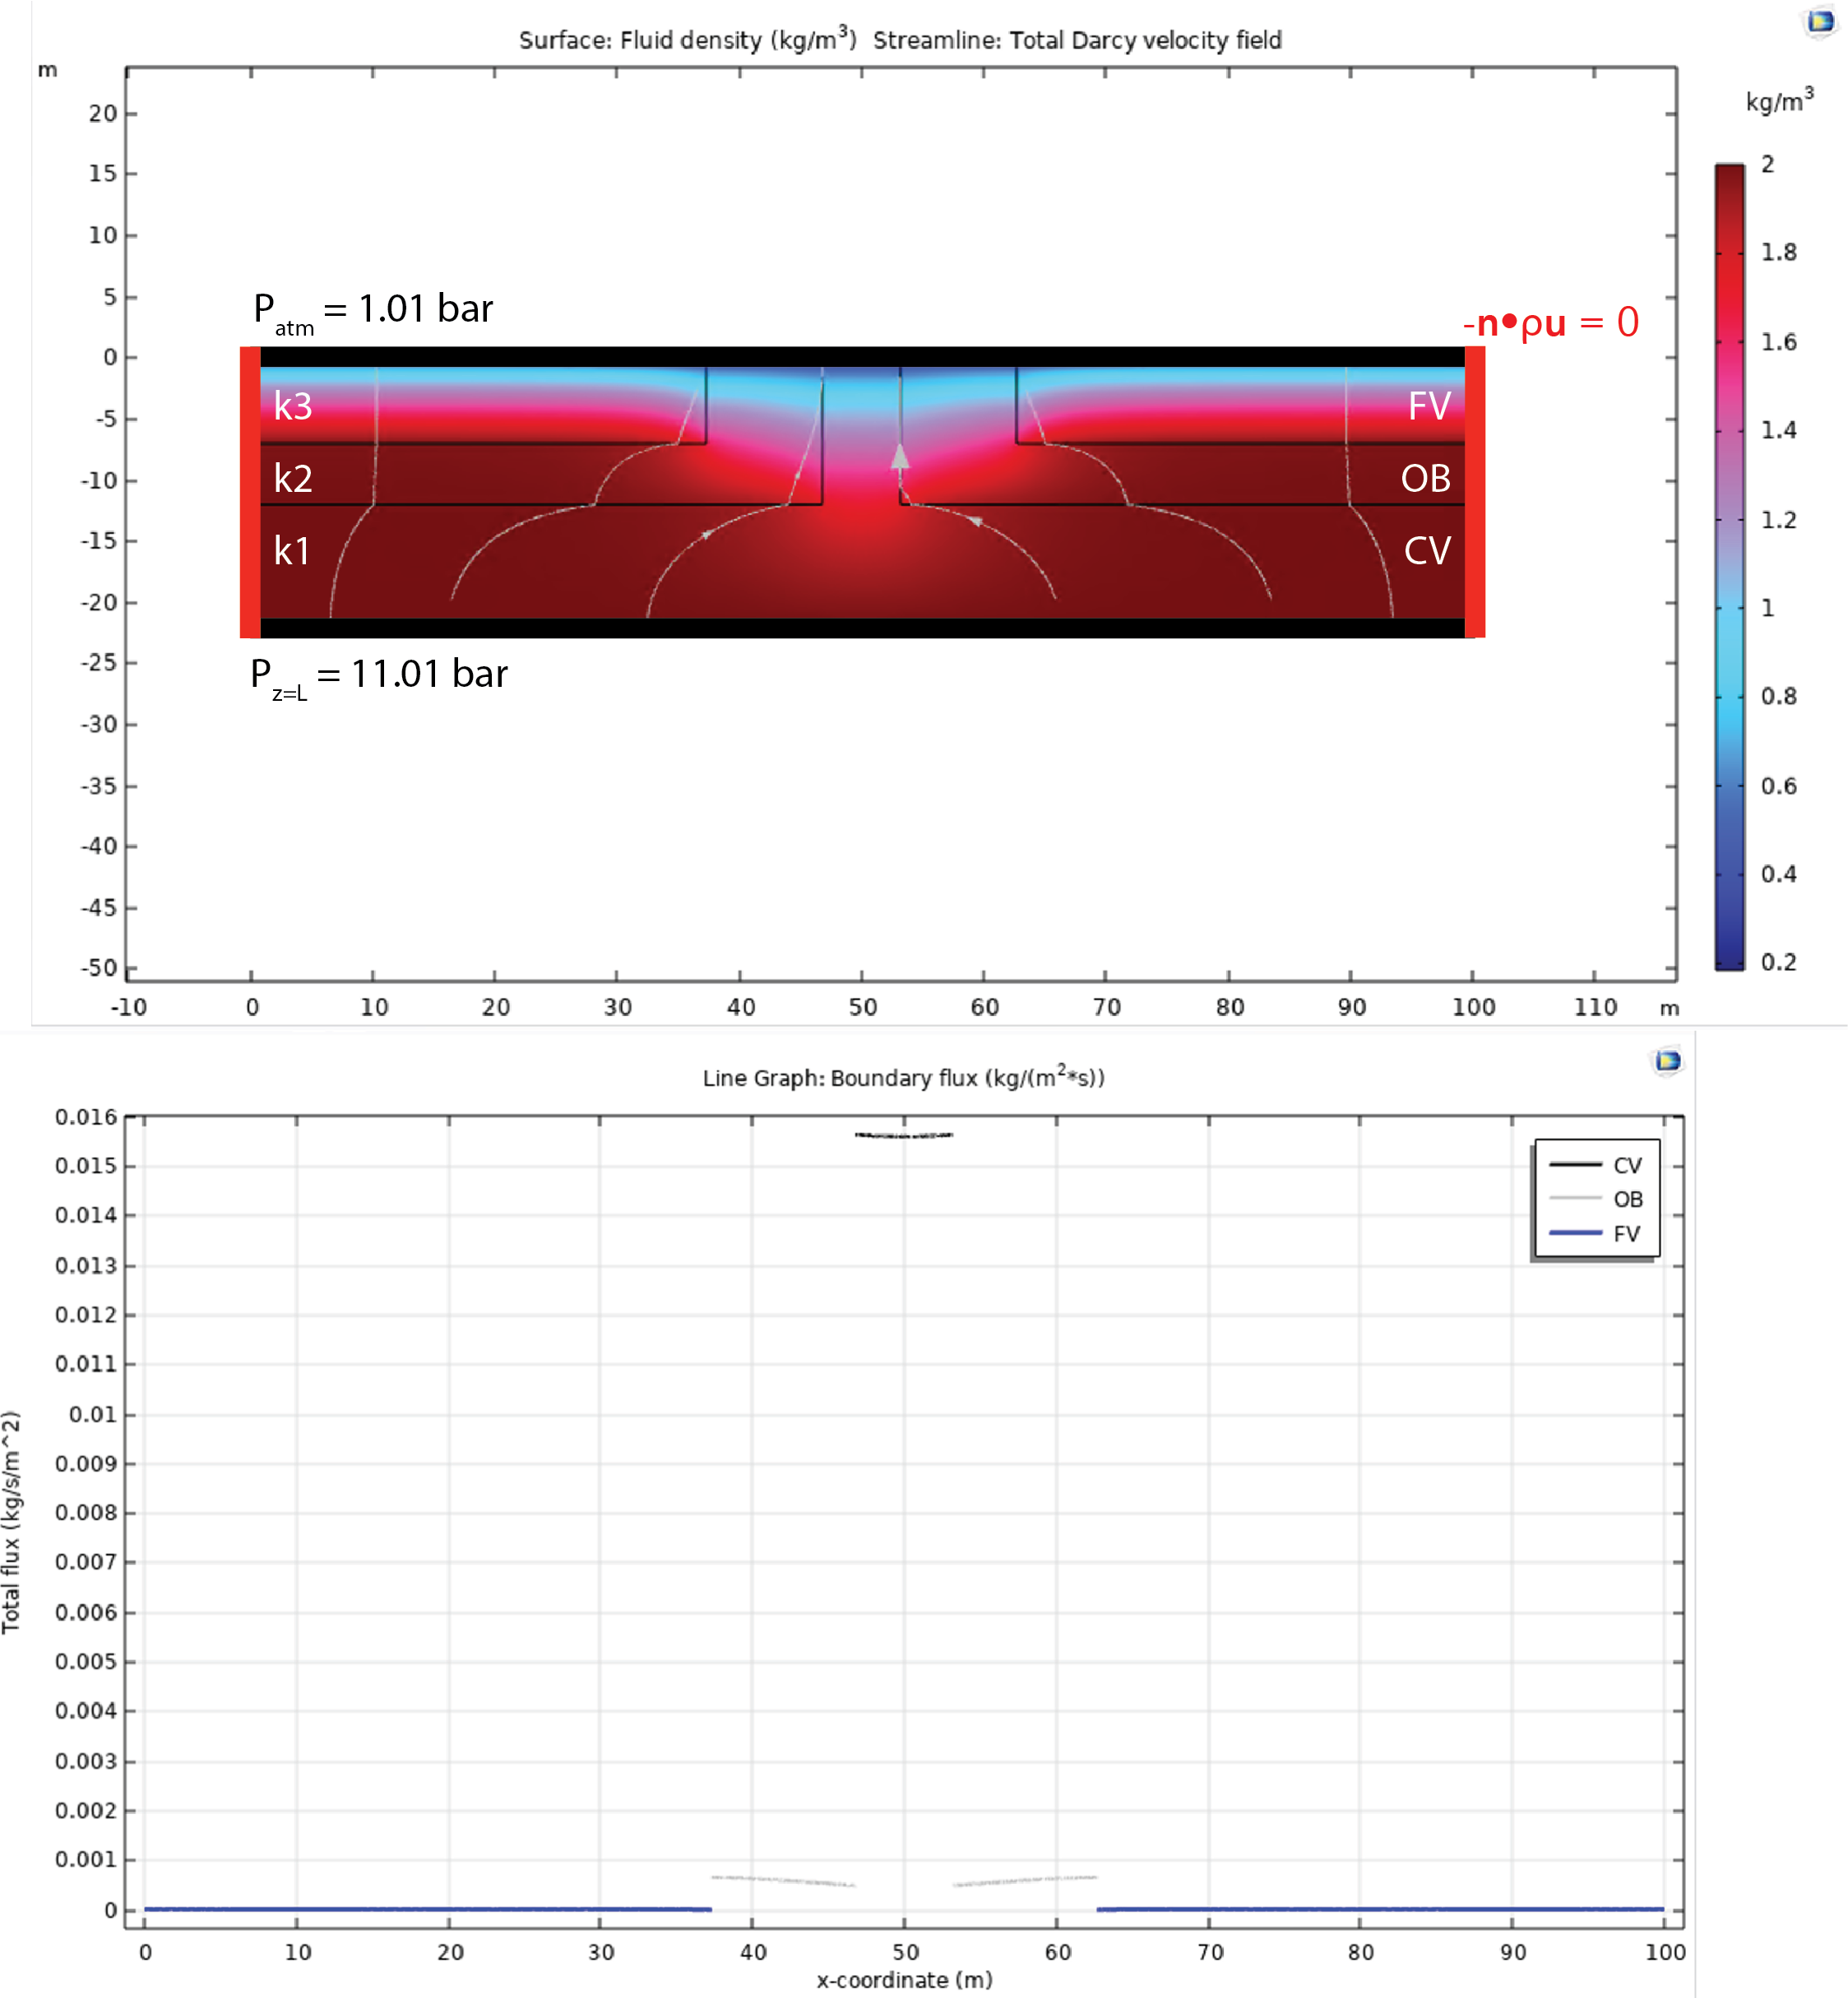
\includegraphics[scale=0.8]{comsolDarcyLaw_units.png}
\caption{Top figure shows gas density in unit layers CV, FV, and OB, with permeabilities k1, k2, and k3, respectively (see Table \ref{tab:UnitPermPoro}). Streamlines indicate the direction of gas flow. Pressure boundary conditions at the base and surface of the units are shown in black, and no flow boundary conditions at the side of the units are shown in red. The bottom figure shows the gas flux at the surface.}
\label{fig:COMSOLresults}
\end{figure}


\begin{table}[h]
\center
      \small
      \begin{tabular}{lllll}
      \hline
      \textbf{Unit} & \textbf{Permeability (m\textsuperscript{2})} & \textbf{Connected porosity (\%)}  & \textbf{Height (m)} & \textbf{Percent of total dome surface area} \\  
      \hline
      CV & 6.87E-12 & 50.0 & 10 & 6.4 \\
      FV & 2.18E-13 & 23.2 &  7 & 74.6 \\
      OB & 4.94E-15 & 3.24 & 5 & 19.0 \\ 
\end{tabular}%}
\caption{Average permeability, porosity, height, and percent of total dome surface area of each textural unit.} 
\label{tab:UnitPermPoro}
\end{table}

\printbibliography

\end{document}
